\chapter{Background}
\label{chapter:Background}

This chapter provides an overview of the relevant background information to this thesis. This chapter centres on the chosen greenhouse model and the rationale behind its selection. It examines the principles of RL and MPC, and finally provides an overview of combining these algorithms. 

\section{Greenhouse Model}
\label{section:greenhouse-model}

The accuracy and complexity of a model directly impacts the quality of the control policy.  The dynamics of a greenhouse can be characterised by various modelling approaches depending on its application. Methods such as computational fluid dynamics (CFD) are used to develop numerical models of the indoor climate of a greenhouse using partial differentiable equations. In recent years, CFD simulations have become increasingly more accurate in simulating indoor greenhouse climates \cite{delatorre-geaComputationalFluidDynamics2011}; however, these models are highly complex and require significant computational resources in simulation and optimisation tasks.
Their complexity makes them intractable for mathematical solvers such as MPC, and they present substantial challenges to learning model-free methods, resulting in a demanding and laborious training process \cite{jansenOptimalControlLettuce2023}. 
Simplified models, such as mechanistic models, of greenhouse dynamics are developed by assuming homogeneity in the greenhouse climate and assumptions about $CO_2$ and humidity are made to yield a model conducive to  control applications, as discussed in \citet{jansenOptimalControlLettuce2023, lopez-cruzDevelopmentAnalysisDynamical2018}. These mechanistic process models are often derived from first principles and use ordinary differential of difference equations to represent the system dynamics. While these mechanistic models sacrifice some accuracy in representing the system, they significantly reduce computational demands, often making them tractable for mathematical solvers. 
In contrast, data-driven models such as in \citet{gongDeepLearningBased2021} and \citet{maestriniMixingProcessbasedDatadriven2022} have also been used to create a black box model of the greenhouse dynamics. Although such models may yield accurate results, they do so only in the environment from where the data originates. Mechanistic process models often generalise better to different environments and situations. While such black box models could be used for RL, they could pose challenges for mathematical solvers due to their potential complexity and unknown mathematical makeup.
\\
Although accurate models may seem appealing, they are often complex and entail a high-dimensional state space. Both factors adversely affect model-free RL algorithms and MPC, making such models impractical for developing optimal control policies. This arises because, in the case of MPC, finding a tractable solution in the given time constraints may prove challenging. This can results in failure to meet timing requirements and constraints, or find no solution. Similarly, in model-free RL algorithms, using highly accurate models could destabilise the learning procedure, making it a more complex and time-consuming task to learn a policy \cite{lawrynczukMPCAlgorithms2014,dulac-arnoldChallengesRealWorldReinforcement2019}. Therefore, for optimal control, it is desirable to use a low-dimensional simplified model whereby the most critical dynamics of the system are still captured. Moreover, the control law obtained from the simplified model may be adjusted and applied to the more accurate models to validate them. However, if the control law is unsatisfactory, the simplified model must be adapted, and a new control policy obtained. Often, this leads to an iterative cycle of updating the model and validating the control policy until a satisfactory performance of the high-accurate model is obtained \cite{knibbeDigitalTwinsGreen2022}. Since this thesis focuses on the impact and implementation of merging RL and MPC for optimal control, designing and developing a model is outside the scope.
Therefore, a validated simplified mechanistic model of a greenhouse with lettuce crops will be selected.
Due to the relative simplicity of lettuce crop models, they find utility alongside a greenhouse model that assumes an indoor homogeneous climate. A model that encapsulates the fundamental dynamics of the greenhouse and crops is detailed in \citet{hentenGreenhouseClimateManagement1994} and has been explicitly developed for optimal control applications. More importantly, the propsed model in \citet{hentenGreenhouseClimateManagement1994} has been validated in \citet{vanhentenValidationDynamicLettuce1994}, and has been extensively used in obtaining optimal control policies such as in \citet{jansenOptimalControlLettuce2023,vanstratenOptimalGreenhouseCultivation2010,ghoumariNonlinearConstrainedMPC2005,lubbersAutonomousGreenhouseClimate2023, morcegoReinforcementLearningModel2023}. Therefore, the choice was made to use the model suggested in \citet{hentenGreenhouseClimateManagement1994} for this thesis.



\subsection{Model Description}
\begin{figure}[H]
	\centering
	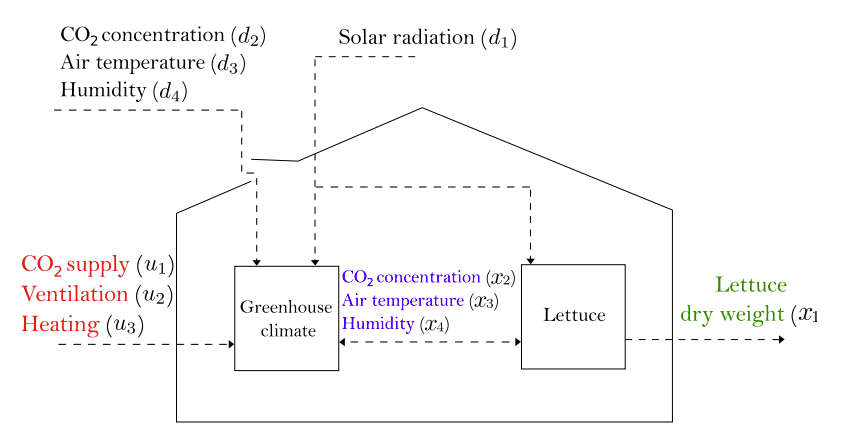
\includegraphics[width = 0.75\linewidth]{figures/van_henten_model.png}
	\caption{Graphical representation of greenhouse crop production \cite{hentenGreenhouseClimateManagement1994}}
	\label{fig:van_henten_model}
\end{figure}

\autoref{fig:van_henten_model} displays a graphical representation of the greenhouse model from the works of \citet{hentenGreenhouseClimateManagement1994}. The control inputs are highlighted in red, the states of the indoor climate in blue, the state of the crop in green and the external disturbances in black. The states of the system, control inputs, disturbances and outputs are described in \autoref{eq: model vectors}.

\begin{equation}
	\begin{aligned}
		& x(k) = \begin{bmatrix}
			x_1 & x_{2} & x_3 & x_4
		\end{bmatrix}^T
		\\
		& u(k) = \begin{bmatrix}
			u_{1} & u_{2} & u_3
		\end{bmatrix}^T
		\\
		& d(k) = \begin{bmatrix}
			d_{1} & d_{2} & d_3& d_4
		\end{bmatrix}^T
		\\
		& y(k) = \begin{bmatrix}
			y_1 & y_{2} & y_3 & y_{4}
		\end{bmatrix}^T
	\end{aligned}
	\label{eq: model vectors}
\end{equation}

The state of the system includes crop dry mass, indoor $C0_2$ density, temperature and the absolute humidity. Crop dry mass is used since it is a more reliable and accurate measure of the plant's biomass. Unlike fresh weight, which varies with the plant's water content and is influenced by weather conditions, crop dry mass provides a more stable and consistent metric. The control vector encapsulates the $C0_2$ injection and ventilation rate and the heating supply. Furthermore, the disturbances from the weather include the incoming solar radiation, outside $C0_2$ density, temperature and the outside humidity. The measured output is essentially the same as the state of the system; however, the units of the indoor $C0_2$ density ($y_2$) and relative humidity ($y_4$) differ in that they report in units used in standard measurement sensors. The non-linear continuous-time dynamics is represented by \autoref{eq:greenhouse_model_continous}

\begin{equation}\label{eq:greenhouse_model_continous}
	\begin{aligned}
		& \dot{x}= f(x(t),u(t),d(k),p) \\
		& y(k) = g(x(k),u(k),d(k),p)
	\end{aligned}
\end{equation}

where $p=\mu_p$ and $\mu_p$ is the value of all the parameters used in the model and displayed in \autoref{tab:model constants and descriptions}, $x$ is the model state, $y$ is the measurement outputs and $d$ is the weather disturbance. The next section examines the model's state equations in more depth.

\subsection {Model State Equations}

\paragraph{State Equations}
The model described in \cite{hentenGreenhouseClimateManagement1994} is fully described by the crop dry weight, temperature, humidity and $C0_2$ levels of the indoor climate. All variables and their units are given in \autoref{tab:model variables and descriptions} and model constants in \autoref{tab:model constants and descriptions}. These states are modelled using a set of ordinary differentiable equations given below:

\begin{equation}
	\frac{dx_1}{dt} = c_{\alpha \beta} \phi_{phot,c}(t) - \phi_{resp,d}(t)
\end{equation}

\begin{equation}
	\frac{dx_{2}}{dt} = \frac{1}{c_{cap,c}}(-\phi_{phot,c}(t) + \phi_{resp,c}(t) + u_{C0_2}(t) \cdot 10^{-6} - \phi_{vent,c}(t))
\end{equation}

\begin{equation}
	\frac{dx_{3}}{dt} = \frac{1}{c_{cap,q}}(u_{q}(t) - Q_{vent,q}(t) + Q_{Io,q}(t))
\end{equation}

\begin{equation}
	\frac{dx_{4}}{dt} = \frac{1}{c_{cap,h}}(\phi_{transp,h}(t) - \phi_{vent,h}(t))
\end{equation}

where parameter values,units and descriptions can be found in \autoref{tab:model constants and descriptions}. The process equations, denoted as $\phi(\cdot)$ are described in \autoref{tab:model variables and descriptions} and are represented by the following set of equations:
\begin{equation}
	\phi_{phot,c}(t) = (1 - e^{-C_{LAI,d} x_d(t)}) \frac{c_{Io}^{phot} d_{Io}(t) \cdot \phi(t)}{c_{Io}^{phot} d_{Io}(t) +\phi(t)}
	\label{eq: canopy photosynthesis rate}
\end{equation}

\begin{equation}
	\phi (t) = ( -c_{C0_2,1}^{phot} x_T(t)^2 +  c_{C0_2,2}^{phot} x_T(t) - c_{C0_2,3}^{phot} )( x_{C0_2}(t) - c^{phot})
	\label{eq: model phi}
\end{equation}

\begin{equation}
	\phi_{resp,d}(t) = c_{resp,d} \cdot \phi_{resp}(t)
	\label{eq:maintenance respiration rate}
\end{equation}

\begin{equation}
	\phi_{resp}(t) = x_d(t) \cdot c_{Q_{10},resp}^{(x_T(t)-25)/10}
	\label{ respiration maintenance}
\end{equation}

\begin{equation}
	\phi_{resp,c}(t) = c_{resp,C0_2} \cdot \phi_{resp}(t)
	\label{ co2 respiration rate}
\end{equation}

\begin{equation}
	\phi_{vent,c}(t) = (u_v(t) \cdot 10^{-3} + c_{leak})(x_{C0_2}(t) - d_{C0_2}(t))
	\label{eq:co2 exchange}
\end{equation}

\begin{equation}
	Q_{vent,q}(t) = (c_{cap,v}u_v(t) + c_{go})(x_T(t) - d_T(t))
	\label{heat exchange}
\end{equation}

\begin{equation}
	Q_{I_o,q}(t) = c_{og}^{rad} d_{I_o}(t)
\end{equation}

\begin{equation}
	\phi_{transp,h}(t) = c_{ca}^{evap}(1 - e^{-C_{LAI,d} x_d(t)})\cdot \left( \frac{c_{H_2O,1}^{sat}}{c_R(x_T(t)+c_T)} e^{\frac{c_{H_2O,2}x_T(t)}{x_T(t) + c_{H_2O,3}}} - x_h(t) \right)
\end{equation}

\begin{equation}
	\phi_{vent,h}(t) = (u_v(t) \cdot 10^{-3} + c_{leak})(x_h(t) - d_h(t))
\end{equation}

\paragraph{Output Measurement Equations}
The output measurements for the indoor humidity and $C0_2$ levels are reported in different units via the function $g_{C0_2}(\cdot)$ and $g_h{\cdot}$ respectively.  The output measurements for crop dry mass and indoor temperature correspond to the state variables, as illustrated below:

\begin{equation}
	\begin{aligned}
		& y_1(t) = x_1(t) 
		\\
		& y_{2}(t) = g_{C0_2}(x_3(t),x_{2}(t))
		\\
		& y_3 (t) = x_3(t)
		\\
		& y_{4} = g_h (x_3(t),x_4(t))
	\end{aligned}
\end{equation}

\begin{equation}
	g_{C0_2}(z_T(t),z_{C0_2}(t)) = 10^3 \cdot \frac{R(z_T(t) + c_T)}{PM_{C0_2}} \cdot z_{C0_2}(t)
\end{equation}
\begin{equation}
	g_h (z_T(t),z_h(t)) = \frac{R(z_T(t) + c_T)}{c_{H_20,4}^{sat}\cdot \text{exp}(\frac{c_{H_20,5}^{sat}z_T(t)}{z_T(t) + c_{H_20,6}^{sat}})} \cdot z_{h}(t)
\end{equation}
where $R,c_T,P,M_{C0_2},c_{H_20,4},c_{H_20,5},c_{H_20,6}$ are constants and their descriptions and units given in \autoref{tab:model constants and descriptions}. The greenhouse model was discretized in time to facilitate the use of MPC and RL. The fourth-order Runge Kutta method was used and results in the discrete model below:

\begin{equation}\label{eq:greenhouse_model_discrete}
	\begin{aligned}
		& x(k+1) = f(x(k),u(k),d(k),p) \\
		& y(k) = g(x(k),p)
	\end{aligned}
\end{equation}

\cite{vanstratenUserAcceptedOptimal2000} recommends discretising the van Henten model using a time-step between 15 minutes and 1 hour. Therefore, a time interval of 30 minutes was selected for this study. 
The initial interval of 30 minutes was initially set at 15 minutes. However, this decision was revised due to the excessive computational burden it imposed on the MPC solver, with minimal benefits. Increasing the time step enables an exponential speedup of the simulation of the growing period, while causing only minor deterioration in performance. Consequently, a larger quantity of training episodes could be used to train the RL.


\begin{table}[H]
	\begin{center}
		\begin{tabular}{|c|c|c|c|}
			\hline
			Category & Symbol & Description & units 
			\\ \hline
			State Variables & $x_1$& crop dry matter& $kg \cdot m^{-2}$
			\\
			& $x_{2}$& Indoor $C0_2$ density& $kg \cdot m^{-3}$
			\\
			& $x_{3}$& Indoor air temperature& $^{\circ}C$
			\\
			& $x_{4}$& Indoor absolute humidity content& $kg \cdot m^{-3}$
			\\ \hline
			Control Inputs & $u_{1}$& $C0_2$ injection rate& $mg \cdot m^{-2} \cdot s^{-1}$
			\\
			& $u_{2}$& Ventilation rate& $mm \cdot s^{-1}$
			\\
			& $u_{3}$& Heating supply& $ W \cdot m^{-2}$
			\\ \hline
			Disturbance     & $d_{1}$& Outside irradiation & $ W \cdot m^{-2}$
			\\
			& $d_{2}$& Outdoor $C0_2$ density& $kg \cdot m^{-3}$
			\\
			& $d_{3}$& Outside ambient air temperature& $^{\circ}C$
			\\
			& $d_{4}$& Outside absolute humidity content& $kg \cdot m^{-3}$
			\\ \hline
			Outputs        & $y_1$& Lettuce dry weight& $kg \cdot m^{-2}$
			\\
			& $y_{2}$& Indoor $C0_2$ concentration& $ppm$
			\\
			& $y_{3}$& Indoor air temperature& $^{\circ}C$
			\\
			& $y_{4}$& Indoor relative humidity content& $\%$
			\\ \hline
			Processes       & $\phi_{phot,c}$& Gross canopy rate& $kg \cdot m^{-2} \cdot s^{-1}$
			\\
			& $\phi_{resp,d}$&Respired dry matter from maintenance respiration of the crop& $kg \cdot m^{-2} \cdot s^{-1}$
			\\
			& $\phi_{resp,c}$& Crop $C0_2$ respiration rate & $kg \cdot m^{-2} \cdot s^{-1}$
			\\
			& $\phi_{vent,c}$& Mass exchange of $C0_2$ between indoor and outdoor climate & $kg \cdot m^{-2} \cdot s^{-1}$
			\\
			& $Q_{vent,c}$& Heat energy exchange  between indoor and outdoor climate & $W \cdot m^{-2}$
			\\
			& $Q_{I_o,q}$& Incoming heat energy from outside irradiation & $W \cdot m^{-2}$
			\\
			& $\phi_{transp,h}$& Canopy transpiration rate & $kg \cdot m^{-2} \cdot s^{-1}$
			\\
			& $\phi_{vent,h}$& Mass exchange of water vapour between indoor and outdoor climate & $kg \cdot m^{-2} \cdot s^{-1}$
			\\ \hline
			
			
		\end{tabular}
	\end{center}
	\caption{Model Variables}
	\label{tab:model variables and descriptions}
\end{table}

\begin{table}[H]
	\centering
	\begin{tabular}{|c|c|c|c|}
		\hline
		Symbol & Description & Value & units 
		\\ \hline
		$c_{\alpha \beta}$& Yield factor &0.544 &-
		\\
		$c_{cap,c}$& Volumetric $C0_2$ capacity of indoor air & 4.1& $m^3 [\text{air}] \cdot m^{-2} [\text{gh}]$
		\\
		$c_{cap,q}$& Effective heat capacity of indoor air &30000 & $J \cdot m^{-2} [\text{gh}] \cdot ^{\circ}C$
		\\
		$c_{cap,h}$&Volumetric humidity  capacity of indoor air & 4.1& $m^3 [\text{air}] \cdot m^{-2} [\text{gh}]$
		\\
		$c_{LAI,d}$&Effective canopy surface & 53& $m^{-2} [\text{L}] \cdot kg^{-1} [\text{dw}]$
		\\
		$c_{I_o}^{phot}$&Light use efficiency & $3.55 \cdot 10^{-9}$& $kg [C0_2] \cdot J^{-1}$
		\\
		$c_{C0_2,1}^{phot}$& Influences temperature gross canopy photosynthesis& $5.11 \cdot 10^{-6}$ & $m \cdot s^{-1} \cdot ^\circ C^{-2}$
		\\
		$c_{C0_2,2}^{phot}$& Influences temperature gross canopy photosynthesis& $2.30 \cdot 10^{-4}$& $m \cdot s^{-1} \cdot ^\circ C^{-1}$
		\\
		$c_{C0_2,3}^{phot}$&Influences temperature gross canopy photosynthesis &$6.29 \cdot 10^{-4}$ &$m \cdot s^{-1}$
		\\
		$c^{phot}$& Carbon dioxide compensation point &$5.2 \cdot 10^{-5}$ &$kg [C0_2] \cdot m^{-3} [\text{air}]$
		\\
		$c_{resp,d}$&Respiration rate of the dry crop matter & $2.65 \cdot 10^{-7}$& $s^{-1}$
		\\
		$c_{Q_{10,resp}}$& Maintenance respiration factor &2 &-
		\\
		$c_{resp,c}$& $C0_2$ release rate factor from respiration &$4.87 \cdot 10^{-7}$ & $s^{-1}$
		\\
		$c_{leak}$& Greenhouse cover ventilation leakage&$7.5 \cdot 10^{-6}$ & $m \cdot s^{-1}$
		\\
		$c_{cap,v}$& Heat capacity of indoor temperature per volume & 1290 & $J \cdot m^{-3} [\text{gh}] \cdot ^\circ C^{-1}$
		\\
		$c^{go}$& Heat transmission through cover factor &6.1 &$W \cdot m^{-2} [\text{gh}] \cdot ^\circ C^{-1}$
		\\
		$c_{og}^{rad}$&Solar heat load coefficient & 0.2&-
		\\
		$c_{ca}^{evap}$&Vapour mass transfer factor between leaf and air  & $3.6 \cdot 10^{-3}$ & $m \cdot s^{-1}$
		\\
		$c_{H_20,1}^{sat}$& Influences water vapour saturation point&9348 & $J \cdot m^{-3}$
		\\
		$c_{H_20,2}^{sat}$&Influences water vapour saturation point &17.4 & -
		\\
		$c_{H_20,3}^{sat}$& Influences water vapour saturation point&239 & $^\circ C$
		\\
		$c_{H_20,4}^{sat}$& Influences water vapour saturation point&610.48 & Pa
		\\
		$c_{H_20,5}^{sat}$&Influences water vapour saturation point &17.2694 & -
		\\
		$c_{H_20,6}^{sat}$& Influences water vapour saturation point&238.3 & $^\circ C$
		\\
		$c_R$& Gas constant &8314 & $J \cdot K^{-1} \cdot \text{kmol}^{-1}$
		\\
		$c_T$& For conversion between Kelvin and Celsius &273.15 & K
		\\
		$R$&Molar gas constant &8.3144598 &$J \cdot \text{mol}^{-1} \cdot K^{-1}$
		\\
		$P$&Pressure at 1 atmospheric pressure &101325 & Pa
		\\
		$M_{C0_2}$& Molar mass of $C0_2$ &0.0441 & $kg \cdot \text{mol}^{-1}$
		\\
		\hline
	\end{tabular}
	\caption{Model Constants}
	\label{tab:model constants and descriptions}
\end{table}

\subsection{Model uncertainty}
In reality, uncertainty is present in all aspects of the model. In the case of the greenhouse environment, uncertainty may arise in the weather predictions, there may be measurement noise on the outputs and the control inputs may not be exact. Additionally, the simplified model leads to a model mismatch, which may result in significant prediction errors.  As was done in \cite{boersmaRobustSamplebasedModel2022, lubbersAutonomousGreenhouseClimate2023}, the source of uncertainty in the stochastic environment is modelled as parametric uncertainty, which aims to capture all the uncertainty in the greenhouse environment. Moreover, in the objective function (discussed further in \autoref{ssection:optimization-goal}), the pricing of energy and the lettuce may also be stochastic. However it is assumed to be fixed, along with the weather predictions.
This thesis does not focus on accurately modelling the uncertainty in a greenhouse crop environment. However, it is essential to observe the impact of uncertainty on the policy generated for each algorithm. This will help determine the performance of these controllers in a more realistic scenario. Thus, the parameters of the environment are represented as uncertain with well-defined probabilistic properties. It is assumed that the uncertain parameters, $\hat{p}$, follow the uniform probabilistic distribution:
\begin{equation}
	\label{eq:uncertainty_model}
	\begin{aligned}
		\hat{p} \sim U(\mu_p, \delta_p)  
	\end{aligned}
\end{equation}
where $\mu_p = p$ is the mean value of the parameters  (shown in \autoref{tab:model constants and descriptions}) and $\delta_p$ are expressed as a percentage where the upper and lower bounds of the distribution is expressed as $p(1-\delta_p)$ and $p(1+\delta_p)$. It must be noted that since all parameters are perturbed, including parameters of the output measurement equations, output noise is also introduced. The uniform distribution was chosen for its higher level of aggression compared to the normal distribution. While it may not accurately represent the uncertainty at hand, it is  useful for evaluating the potential variability and risks associated with the various policies, especially at higher degrees of uncertainty. Introducing this uncertainty results in the following system dynamics:

\begin{equation}\label{eq:greenhouse_model_discrete_uncertain}
	\begin{aligned}
		& \hat x(k+1) = f(\hat x(k),u(k),d(k),\hat p(k)) \\
		& \hat y(k) = g(\hat x(k),\hat p(k))
	\end{aligned}
\end{equation}

where the states and output measurements of the system are uncertain and $\hat{p}(k)$ denotes the uncertain parameters and is resampled at every time step.



\subsection{Optimisation Goal}
\label{ssection:optimization-goal}
Maximising the economic profit of the greenhouse is highly desirable. This concept involves maximising the lettuce's size while minimising the resources used throughout its entire growth period. The optimisation goal can be modeled and is referred to by the economic profit indicator (EPI), as demonstrated below:

\begin{equation}\label{eq:epi}
	EPI = \sum_{k = ts}^{tf} (c_{p_1} \cdot u_1(k) + c_{p_2} \cdot u_3(k))\cdot \Delta t - c_{p_3} \cdot y_1(tf)
\end{equation}

where $t_s$ denotes the starting time, $t_f$ the end time, $\Delta t$ the time interval,$c_{p1},c_{p2}$ the pricing coefficients of injecting $C0_2$, and heating, respectively and $c_{p3}$ as the price of lettuce. These pricing factors are shown in \autoref{tab:pricing_factors}. It is important to highlight that ventilation, such as opening windows, does not incur any costs and, therefore, does not have a pricing factor. Although it is also possible to optimise $tf$, i.e. when is the best time to sell the lettuce, it is decided to keep the growing period fixed. The growing period for lettuce typically falls within 30 to 50 days. Therefore, a fixed growing period of 40 days was selected. As a result, over 40 days (1 episode or 1 complete simulation), there is a total of:
$$
k_{total} = \frac{40 \frac{days}{growing \, period} \cdot 24 \frac{hrs}{day} \cdot 60 \frac{min}{hr}}{30 \frac{min}{timestep}} = 1920 \frac{time \, steps}{growing \, period}
$$

Moreover, this optimisation goal is subject to constraints where the control constraints are:

\begin{equation}\label{eq:input constraints}
	\begin{aligned}
		&u_{min} = \begin{pmatrix}
			0&0&0
		\end{pmatrix}^T \\
	&u_{max} = \begin{pmatrix}
		1.2&7.5&150
	\end{pmatrix}^T	\\
& \delta u_{max} = \frac{1}{10} u_{max}
	\end{aligned}
\end{equation}

and the state constraints are defined as:

\begin{equation}\label{eq:state constraints}
	\begin{aligned}
		&y_{min} = \begin{pmatrix}
			0&500&10&0
		\end{pmatrix}^T \\
		&y_{max} = \begin{pmatrix}
			\infty&1600&20&100
		\end{pmatrix}^T	\\
		& \delta_u = \frac{1}{10} u_{max}
	\end{aligned}
\end{equation}

The values in question were obtained from typical horticultural practices. In many papers, such as \citet{boersmaRobustSamplebasedModel2022}, the lower and upper boundaries of the indoor temperature are time-varying to aid MPC in making better decisions. It was decided to keep the lower and upper bounds of the temperature constant to give RL and MPC as much freedom for optimizing for an economic benefit.

\begin{table}[H]
	\centering
	\begin{tabular}{|c|c|c|}
		\hline
		\textbf{Symbol} & \textbf{Value} & \textbf{Units} \\
		\hline
		$c_{p_1}$ & $1.906\cdot 10^{-7} \times 10^{-4}$ & $ \cdot \text{\euro} \cdot mg^{-1}$ \\
		$c_{p_2}$ & $3.558 \times 10^{-8}$ & $ \text{\euro} \cdot J^{-1}$ \\
		$c_{p_3}$ & $22.285$ & $\text{\euro} \cdot kg^{-1}$ \\ 
		\hline
	\end{tabular}
	\caption{Pricing factors}
	\label{tab:pricing_factors}
\end{table}


The pricing factors accounts for the required conversions from $mg$ to $kg$ and joules to $kWh$ for the $C02$ injection and heating, respectively. Furthermore, $c_{p_3}$ incorporates the factor of harvestable fresh weight, which quantifies the amount of fresh relative to dry weight. Finally, the pricing of the $C0_2$ in \euro $/kg$, the price of heating in \euro$/kWh$ and the pricing of lettuce in \euro$/kg$ is also incorporated as shown in \autoref{eq:pricing factors}

\begin{equation}\label{eq:pricing factors}
	\begin{aligned}
		& c_{p1} = C0_{2_{price}}  =  \frac{0.1906 \frac{\text{\euro}}{kg}}{10^{6} \frac{mg}{kg}}\\
		& c_{p2} = \text{Heating}_{price} = \frac{0.1281 \frac{\text{\euro}}{kWh}}{3.6\cdot 10^{6} \frac{J}{kWh}}\\
		& c_{p3} = (1-c_{\tau})  \cdot c_{fw} \cdot Let_{price}= (1-0.07) \cdot 22.5 \frac{kg_{fw}}{kg_{dw}} \cdot 1.065 \frac{\text{\euro}}{kg} \\
	\end{aligned}
\end{equation}

The prices for $C0_{2_{price}}$, $\text{Heating}_{price}$, and $Let_{price}$ were sourced from \cite{vandenbemdRobustDeepReinforcement}, while the factors for harvestable fresh weight, $c_{\tau}$ and $c_{fw}$, were obtained from \cite{hentenGreenhouseClimateManagement1994}. While these factors may not accurately reflect the present economic conditions, it is important to keep them constant when comparing the MPC, RL, and RL-MPC algorithms. This ensures a meaningful comparison between algorithms, which aligns with one of the objectives of this thesis. As shown in \autoref{eq:epi}, this optimisation goal makes the reward incredibly sparse, making it difficult to optimise directly with both MPC and RL. Consequently, both algorithms use a stage cost received at every time interval, whereby the total sum of these stage costs throughout the growing period corresponds to the optimisation objective in \autoref{eq:epi}. Therefore the optimisation goal that RL, MPC and RL-MPC aims to optimise is:

\begin{equation}\label{eq:stage-cost-epi}
	\min_{u_1,u_3} \sum_{k = ts}^{tf} {(c_{p_1} \cdot u_1(k) + c_{p_2} \cdot u_3(k))\cdot \Delta t - c_{p_3} \cdot (y_1(k) - y_1(k-1)) }
\end{equation}


 \cref{section:env-description} and \cref{section: greenhouse MPC formulation} further discuss the implementation of \autoref{eq:stage-cost-epi} for RL and MPC, respectively.


\section{Reinforcement Learning}\label{section:RL}

With the surge in AI development, the demand for optimal greenhouse control has brought RL into the spotlight. Although AI algorithms are already used in farming and horticulture, most applications are centred on detecting and protecting plant and crop quality, such as plant stress, pests and disease and weed detection \cite{hemmingCherryTomatoProduction2020}. Moreover, the prediction of crop yield and growth has also been a focus area for AI owing to its unparalleled non-linear approximation capabilities \cite{gongDeepLearningBased2021}. Additionally, recent advances in RL have displayed its ability to outperform humans in decision-making when presented with sizeable complex problem spaces \cite{bonsaiWhyReinforcementLearning2017}. Because of RL's ability to evaluate optimal control actions for large state spaces, it has shown great success, such as in Google DeepMind's chess engine, AlphaZero, creating one of the most powerful chess engines in the world. Furthermore, reinforcement learning has demonstrated exceptional proficiency in handling uncertainty and disturbances \cite{daaboulUncertaintyPredictionModelbased2020}. This makes it an ideal control strategy for greenhouse management, particularly considering the uncertainties inherent in weather conditions and crop growth. \\

Recently, research has focused on optimising crop growth and yield in greenhouse control, with studies such as \cite{ajagekarDeepReinforcementLearning2022,wangDeepReinforcementLearning2020,ajagekarEnergyefficientAIbasedControl2023,decardi-nelsonbenjaminImprovingResourceUse2023,zhangRobustModelbasedReinforcement2021,jansenOptimalControlLettuce2023,vanmourikPlantPerformancePrecision2023} employing reinforcement learning to address this challenge. This momentum has been fueled by initiatives like the Autonomous Greenhouse Challenge hosted by Wageningen University and Research, first held in 2018, in which the challenge was designed to push the limits of AI in fresh food production. In this competition, teams vie against each other to employ AI to optimise cucumber crops in a climate-controlled greenhouse. Specifically, deep reinforcement learning policies have been applied and measured against each other, as well as current control strategies and expert growers, showing promising results and, in some cases, outperforming expert growers \cite{vandenbemdRobustDeepReinforcement,wangDeepReinforcementLearning2020}. As the years have progressed, more teams have succeeded in outperforming expert growers \cite{vandenbemdRobustDeepReinforcement,hemmingCherryTomatoProduction2020}. Such achievements using reinforcement learning in a real-world application have displayed its potential to achieve complete autonomous greenhouse control.

\subsection{The RL problem}
Reinforcement Learning consists of four main components that define its nature: a policy, a reward signal, a value function and a representation of the environment \cite{suttonReinforcementLearningIntroduction2014}. To further conceptualize the idea of RL, there exists an agent,environment and a reward signal that outlines the goal of the optimization problem (\autoref{fig:agent_environment}).This agent explores and takes actions in the environment where at time $k$ follows a policy $\pi_{k}$ and the agent receives a reward $R_{k}$ from the environment based on the action taken and the state of the agent. This policy is defined as a control law that maps the agent's states to probabilities of selecting each possible action that an agent can take \cite{suttonReinforcementLearningIntroduction2014}. The only objective of the agent is to maximize the cumulative reward of the agent, therefore the agent learns to make decisions and take actions that lead to favourable outcomes, as measured by the received rewards in the environment. Finally, the value function is defined as the expected future rewards based on the current state of the agent. Therefore the reward received is a measure of the immediate desire for an state, and the value function indicates the long-term desirability of a state. \cite{suttonReinforcementLearningIntroduction2014}.\\

This interaction between agent and environment in Reinforcement Learning is modeled as a Markov Decision Process (MDP). This mathematical framework formalizes the decision process that satisfies the condition whereby future states depend only on the current state and action taken. The agent-environment interaction is as shown in \autoref{fig:agent_environment} and depicts the agents taking actions $A_t$ in the environment and receiving reward $R_{t+1}$ and transitioning to the next state $S_{t+1}$ with probability $P$ at every discrete time step $k$.



%discuss markov chains and properties
\begin{figure}[h]
	\centering
	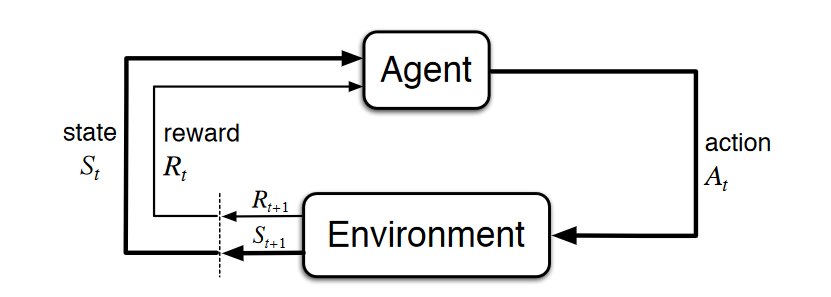
\includegraphics[width=0.75\linewidth]{figures/agent-environment.png}
	\caption{Agent-Environment interaction \cite{suttonReinforcementLearningIntroduction2014}}
	\label{fig:agent_environment}
\end{figure}

The MDP problem can be characterized as a tuple of states, actions, rewards and a state transition function. Such that:

\begin{itemize}
	\item states: ($S_t\in \mathcal{S}$) where $\mathcal{S}$ is the finite state space.
	\item Actions: ($A_t \in \mathcal{A}$) where $\mathcal{A}$ is the finite action space.
	\item Transition probability: $P(S_{t} = s',R_{t} = r | S_{t-1} = s, A_{t-1} = a)$ where $P(\cdot)$ represents the probability of transitioning to state $s'$ and receiving reward $r$ given the previous state and action. This defines the dynamics of the MDP.
	\item Rewards: $r:\mathcal{S}\times \mathcal{A} \rightarrow \mathbb{R}$ where $r(s,a) = \mathbb{E}[R_{t}| S_{t-1} =s, A_{t-1} = a]$  is the reward function.
\end{itemize}


Furthermore, the agent follows a policy $\pi$ that establishes a mapping from states to actions, $\pi: S_t \rightarrow A_t$. The optimal policy seeks to maximize the total expected return (cumulative reward) of the agent where the return, $G_t$, is defined as some specific function of the reward sequence \cite{suttonReinforcementLearningIntroduction2014} as shown in \autoref{return_function}. 
\begin{equation}
	\begin{aligned}
		G_t  = R_{t+1} + R_{t+2} + R_{t+3} + \dots + R_{T} = \sum_{k=0}^TR_{t+k+1}
	\end{aligned}
	\label{return_function}
\end{equation}
However this is only relevant for scenarios where there is a time horizon and/or an idea of a final time step $T$ such as a task with some defined end point or events that are episodic in nature. This does not however extend to problem that does not necessarily follow naturally identifiable episodes, and therefore the notion of an infinite time horizon with discounted returns is introduced. Where the return function now becomes:

\begin{equation} \label{eq:total-return}
	\begin{aligned}
		G_t  = R_{t+1} + \gamma R_{t+2} + \gamma^2 R_{t+3} + \dots = \sum_{k=0}^\infty \gamma^k R_{t+k+1} = R_{t+1} + \gamma G_{t+1}
	\end{aligned}
\end{equation}

and the discount factor $\gamma \in [0,1]$. Although the return (\autoref{eq:total-return}) is a sum of an infinite number of terms, it is still finite if $\gamma < 1$ \cite{suttonReinforcementLearningIntroduction2014}. As the discount factor, $\gamma$, approaches one, the more future rewards are considered.  In contrast, values approaching zero render the agent "myopic", focusing solely on maximizing immediate rewards. The discount factor, $\gamma$, commonly fall within the range of 0.9 to 0.995 \cite{vandenbemdRobustDeepReinforcement}. This is an important concept since it can be shown that if the rewards are bounded (i.e. $\in \mathbb{R}$) and a discount value of $\gamma <1$ is used, then a stable optimal policy can be found \cite{bertsekasNewtonMethodReinforcement2022}. There follows that a value function exists, under a specific policy $\pi$ of a state $s$, denoted as $v_{\pi}$ and defined as the expected return starting in state $s$ and following the policy $\pi$ thereafter. This value function is depicted below in \autoref{value_function}.

\begin{equation}
	\begin{aligned}
		V_{\pi}(s) =  \mathbb{E}_{\pi}\left[{G_t | S_t = s}\right] =  \mathbb{E}_{\pi} 
		\left [\sum_{k=0}^{\infty} \gamma^k R_{t+k+1} | S_t = s \right], \forall s \in \mathcal{S} 
	\end{aligned}
	\label{eq:value_function}
\end{equation}

Given the absence of transition dynamics in a standard RL problem, this can be extended for a state-action pair value function as in \autoref{eq:state-value_function} whereby $Q_{\pi}$ denotes the expected return starting from state $s$ and taking action $a$, under the policy $\pi$ \cite{ajagekarDeepReinforcementLearning2022}.
\begin{equation}
	\begin{aligned}
		Q_{\pi}(s,a) =  \mathbb{E}_{\pi}\left[{G_t | S_t = s, A_t = a}\right] =  \mathbb{E}_{\pi}\left[\sum_{k=0}^{\infty} \gamma^k R_{t+k+1} | S_t = s, At = a\right]
	\end{aligned}
	\label{eq:state-value_function}
\end{equation}

Important to note, that from \autoref{eq:total-return} and \autoref{eq:value_function}, a value function under a generic stationary (does not change over time) policy $\pi$ satisfies the Bellman equation as shown in \autoref{eq:bellman equation for value iteration} \cite{bertsekasNewtonMethodReinforcement2022,bellmanDynamicProgramming1966}.


\begin{equation}
	\begin{aligned}
		V_{\pi}(s) = \mathbb{E} \left[r(s,a) + \gamma V_{\pi}(s') \right] = \mathbb{E} \left[r(s,\pi(s)) + \gamma V_{\pi}(s') \right]
	\end{aligned}
	\label{eq:bellman equation for value iteration}
\end{equation}

Moreover, the value function under the optimal policy, $\pi^*$ can be represented as shown in \autoref{Optimal bellman equation} and for the state-action value function in \autoref{Optimal state-action bellman equation}, where the relation between the value function and state-action value function is shown in \autoref{value and state-action relation} and \autoref{eq:q-function relation to value function}.

\begin{equation}
	\begin{aligned}
		V^*(s) =\max_{a} \mathbb{E} \left[r(s,a) + \gamma V^*(f(x,a)) \right]
	\end{aligned}
	\label{Optimal bellman equation}
\end{equation}

\begin{equation}
	\begin{aligned}
		Q^*(s,a) =\mathbb{E} \left[r(s,a) + \gamma \max_{a'}Q^*(s',a') \right]
	\end{aligned}
	\label{Optimal state-action bellman equation}
\end{equation}

\begin{equation}
	\begin{aligned}
		V^*(s) = \max_{a\in A} Q^*(s, a)
	\end{aligned}
	\label{value and state-action relation}
\end{equation}

\begin{equation}
	\begin{aligned}
		Q^*(s,a) = r(s,a) + \gamma V^*(s') 
	\end{aligned}
	\label{eq:q-function relation to value function}
\end{equation}

Finally, if the optimal state-action value function  (also known as Q-value) is known, then the optimal policy, $\pi^*$ can be found by \autoref{optimal policy} \cite{raoOPTIMALPOLICYOPTIMAL}, whereby the optimal policy greedily selects an action that maximizes the Q-value function.
Various methods exist to approximate this Q-value function; however, it also possible to directly optimize the policy, $\pi$ to find the optimal policy $\pi^*$.

\begin{equation}
	\begin{aligned}
		\pi^*(s) = \arg \max_{a \in A} Q^*(s, a), \forall s \in S
	\end{aligned}
	\label{optimal policy}
\end{equation}

\subsection{Q learning}
These family of algorithms learn an approximating to the Q value function (\autoref{Optimal state-action bellman equation}). Moreover, these algorithms are ``off-policy'' algorithms whereby each update can use data collected at any point during training. Q learning offers a deterministic policy, whereby in each state, the action is selected based on \autoref{optimal policy}. In order to find the optimal Q value function, the update rule in \autoref{eq:q-learning update} is used in combination with a Q-table (a table that holds all possible combinations of discrete states and actions). This iterative update rule aims to approximate the bellman equation in \autoref{Optimal state-action bellman equation}. Once the Q-function converges to the optimal Q-function, the optimal policy can be determined \cite{daveUnderstandingBellmanOptimality2021}.

\begin{equation}
	\begin{aligned}
		Q^{new}(s,a) = (1 -\alpha) \underbrace{Q(s,a)}_{\text{old value}} + \alpha \overbrace{(R_{t+1} + \gamma \max_{a'}(Q(s',a'))}^{\text{Learned value}}
	\end{aligned}
	\label{eq:q-learning update}
\end{equation}

where the temporal difference error is defined as

\begin{equation}
	\begin{aligned}
		TD_{error} = (R_{t+1} + \gamma \max_{a'}(Q(s',a')) - Q(s,a)
	\end{aligned}
	\label{eq:temporal difference}
\end{equation}

where $TD_{error}$ represents the difference between the current Q-value and the target Q-value. When optimality is reached, the TD error is equal to zero, as stated (\autoref{Optimal state-action bellman equation}). However, this is only feasible for finite problems, where the state and action space are small and discrete. In order to accommodate a continuous state space, the Deep-Q Network (DQN) was developed. In this approach, a neural network is utilized to estimate the Q-function, enabling the learning of a deterministic policy from data with high-dimensional features \cite{mnihPlayingAtariDeep2013}. However, DQN still outputs a discrete policy and therefore does not accommodate a continuous action space \cite{mnihPlayingAtariDeep2013}. Nevertheless, recent advancements have extended DQN's applicability to continuous action spaces through the use of actor-critic methods as discussed in \autoref{ssection:actor-critic}.

\subsection{Policy Optimization}
Policy optimization offers a more direct approach in learning the optimal policy as apposed to Q-learning. Such algorithms represent a policy as $\pi_{\theta}(a|s)$, whereby $\pi_{\theta}(a|s)$ is a stochastic policy that gives the probabilities of choosing action $a$ given state $s$. The vector $\theta$ parameterize the policy, and it is these parameters that are optimized, by gradient ascent on the performance objective $J(\theta) = V_{\pi_{\theta}}(s_0)$ such as an \autoref{eq:policy_update}.


\begin{equation}
	\begin{aligned}
		\theta_{t+1} = \theta_{t} + \alpha \hat{\nabla J(\theta_t)}
	\end{aligned}
	\label{eq:policy_update}
\end{equation}

Here, $\hat{\nabla J(\theta_t)}$ represents a stochastic estimate, where its expected value approximates the gradient of the performance objective function with respect to the policy's parameters, $\theta$ \cite{suttonReinforcementLearningIntroduction2014}. Such algorithms are called ``on-policy" algorithms, which mean that each update is performed from data that was collected from the most recent version of the policy.
All RL algorithms that follow this update rule on the policy are considered policy gradient/optimization methods, whether or not they also learn an approximation to a value function. However, such algorithms are often called actor-critic methods \cite{suttonReinforcementLearningIntroduction2014}.  Policy Optimization algorithms are also naturally able to handle continuous state and action spaces.


\subsection{Actor-Critic}\label{ssection:actor-critic}
Perhaps a more interesting class of RL algorithms combines both q-learning and policy optimization. Policy optimisation methods directly optimise the policy and demonstrate superior convergence properties when used in conjunction with function approximators, as opposed to Q-learning. Furthermore, these methods are particularly effective in continuous and stochastic environments when compared to Q-learning \cite{suttonReinforcementLearningIntroduction2014}. However, because Q-learning learns ``off-policy'', it has a substantially higher sample efficiency than that of policy optimizations methods \cite{suttonReinforcementLearningIntroduction2014}.
Actor-critic methods often incorporate the strengths from both policy gradient methods and q-learning, in order to achieve stable and fast learning. The critic learns a value function and the actor learns a policy. The critic provides feedback on how good an action was and uses this to update the policy. In this way, the actor can learn from both its own experience and the critic's feedback 
Moreover, actor-critic algorithms are also suitable in tackling continuous state and action spaces \cite{suttonReinforcementLearningIntroduction2014}. A commonly used actor-critic algorithm  is Soft-Actor-Critic which will be the selected Rl algorithm in this thesis. Numerous actor-critic algorithms exist and for a more in depth explanation on the various algorithms and the decision on why SAC was selected  for this thesis see \autoref{section:RL aglorithms overview} and \autoref{section:selection of RL algorithm} respectively.

\subsection{SAC}
Soft-Actor-Critic (SAC) is an actor critic method that incorporates an entropy term in its reward function to address the trade-off between exploration and exploitation. This results in the agent learning a stochastic policy,$\pi_{\theta}(\cdot|s)$, parametrized by $\theta$, where the entropy term is a measure of randomness in the policy. Consequently, the agent aims to optimise a balance between the total expected reward and entropy, ultimately seeking to maximise rewards while maintaining a policy that is as random as possible. The optimal policy is rewritten as:

\begin{equation}
	\pi^*_{\theta} = \arg \max_{\pi} \mathbb{E} \left[\sum_{t=0}^{\infty} \gamma^t \left( R(s_t, a_t, s_{t+1}) + \alpha H(\pi_{\theta}(\cdot|s)) \right) \right]
\end{equation}


where $H(\cdot)$ is the entropy term and is denoted asand $\alpha > 0$ is called the trade-off coefficient that determines the balance between exploration and exploitation. The entropy of a random variable $x$ with a probability density function $P$ is calculated as:
\begin{equation}
	H(P) = \mathbb{E}_{x \sim P}[-\log P(x)]
\end{equation}

 The value function of a policy $\pi$ is changed to include the entropy term and is denoted as:

\begin{equation}
	V_{\pi}(s) = \mathbb{E} \left[\sum_{t=0}^{\infty} \gamma^t \left( R(s_t, a_t, s_{t+1}) + \alpha H(\pi_{\theta}(\cdot|s)) \right) \,\Bigg|\, s_0 = s \right]
\end{equation}


and the Q-value function as:

\begin{equation}
	Q_{\pi}(s,a) = \mathbb{E} \left[\sum_{t=0}^{\infty} \gamma^t R(s_t, a_t, s_{t+1}) + \alpha \sum_{t=1}^{\infty} \gamma^t H(\pi_{\theta}(\cdot|s)) \,\Bigg|\, s_0 = s, a_0 = a \right]
\end{equation}

Thus the value function is connected to the Q-value function through:

\begin{equation}\label{eq:sac-value-function}
	V_{\pi} (s) = \mathbb{E} \left[Q_{\pi}(s,a) \right] + \alpha H(\pi_{\theta}(\cdot|s))
\end{equation}

The recursive bellman equation of the Q-function of a policy $\pi$, parametrized by $\phi$ becomes:

\begin{equation}
	Q_{\phi}^{\pi_{\theta}}(s,a) = \mathbb{E} \left[ R(s,a,s') + \gamma (Q_{\phi}^{\pi_{\theta}}(s',\bar{a}') - \alpha \log (\pi_{\theta}(\bar{a}'|s')))\right], \quad \bar{a}' \sim \pi_{\theta}(\cdot | s')
\end{equation}

where $s,s',a$ represent the state,next state and action taken respectively and is sampled from the replay buffer. $\bar{a}'$ denotes the action to take in state $s'$ and is sampled using the current policy $\pi_{\theta}(\cdot | s')$. The replay buffer., denoted as $\mathcal{D}$, is used to store the tuple $(s,a,r,s')$ as sampled from the environment based on the agents policy and transitions. A mini batch is uniformly sampled from this replay buffer in order to train the Q-network.

Similarly to DDPG and TD3, SAC uses a clipped double-Q trick with soft updating to learn its Q-value function. The structure of the SAC includes two parametrized Q-functions, $Q_{\phi_1},Q_{\phi_2}$, known as the critics, and one parametrized policy function $\pi_\theta$, known as the actor, where $\phi_1,\phi_2,\theta$ refer to the parameters of its respective neural network. Additionally, each critic has its own target critic with parameters $\phi_{targ,1}$ and $\phi_{targ,2}$ respectively. These target parameters are initialized by copying  $\phi_1,\phi_2$. Unlike in other actor critic algorithms such as mentioned above that train a deterministic policy, the stochastic policy function trained in SAC outputs two vectors describing the mean $\mu_{\theta}$ and the (natural) log standard deviation $\log(\sigma_\theta)$ to determine the policy distribution. However, instead of sampling $\tilde{a}$ directly from this distribution, a reparameterization trick is used where:

\begin{equation}
	\tilde{a}_{\theta} (s, \xi) = \text{tanh} (\mu_{\theta}(s) + \sigma_{\theta}(s) \odot \xi), \quad \xi \sim \mathcal{N}(0,I)
\end{equation}

where $\xi$ is the noise vector and is sampled from a Gaussian distribution and the output squashed between $[-1,1]$ with the tanh function. The greedy deterministic policy (used after training) is then:

\begin{equation}
\pi_{\theta}(s) = \text{tanh}(\mu_{\theta})
\end{equation}

The reparameterization facilitates the learning procedure. The loss function for the Q-networks are defined as:

\begin{equation}
	L(\phi_i,\mathcal{D}) = \mathbb{E} \left[ \left(Q_{\phi_i}(s,a) - y(r,s',d) \right)^2 \right]
\end{equation}

where the target is shared between the two Q-networks and is given by:

\begin{equation}
	y(r,s',d) = r + \gamma (1-d) \left(\min_{j = 1,2} Q_{\phi_{targ,j}}(s', \bar{a}') - \alpha \log (\pi_{\theta} (\bar{a}'|s')))\right), \quad \bar{a}' \sim \pi_{\theta}(\cdot | s')
\end{equation}

The loss function is subsequently minimized by using stochastic gradient descent or a variant of it. The target Q-networks are soft updated by polyak averaging:

\begin{equation}
	\phi_{targ,i} \leftarrow \eta \phi_{i} + (1-\eta)\phi_{targ,i}, \quad i = 1,2
\end{equation}


The policy aims to maximize the expected return and thus the policy loss function becomes:

\begin{equation}
	\max_{\theta} \mathbb{E} \left[\min_{j = 1,2} Q_{\phi_{targ,j}}(s', \tilde{a}_{\theta} (s, \xi)) - \alpha \log (\pi_\theta (\tilde{a}_{\theta} (s, \xi)| s)    \right]
\end{equation}


\section{MPC}\label{section:MPC}
MPC demonstrates exceptional proficiency in managing constrained Multiple Input, Multiple Output (MIMO) systems, making it highly effective in applications like greenhouse control. Moreover, MPC's ability to handle non-linear dynamics and its attempt in achieving optimal control has contributed to its widespread adoption and has become the standard approach for implementing constrained multivariable control in the process industry \cite{daiDiscreteTimeModelPredictive2012}. Nearly every application introduces constraints, whether it be on the state of the system or the control inputs. Actuators, constrained by physical and safety limits such as temperature or pressure control, makes it necessary for controllers to handle such constraints. While the online computational time for such controllers may be expensive, for slow dynamics such as a greenhouse, sufficient computational time may be available to compensate for the extended computational time. Furthermore, the ongoing trend of faster computation mitigates this concern, making it less of a problem.

Although many control schemes exist in controlling greenhouses, it has been shown that an MPC controller outperforms an adaptive PID controller for greenhouse air control in \cite{ghoumariNonlinearConstrainedMPC2005}. Even though the control of a greenhouse is non-linear, using an MPC for control has demonstrated effectiveness in handling this complexity, as evidenced in \cite{gruberNonlinearMPCBased2011, montoyaHybridcontrolledApproachMaintaining2016} specifically for temperature control in a greenhouse. Furthermore, \cite{bersaniModelPredictiveControl2020} shows insight of the performance of MPC when optimized for energy savings of a greenhouse, displaying impressive results over set-point tracking controllers. Further, \cite{boersmaRobustSamplebasedModel2022} successfully implements a robust MPC to control the economic benefit of a greenhouse with parametric uncertainty, displaying its potential in greenhouse control. Moreover, as confirmed by \cite{bersaniModelPredictiveControl2020}, MPC stands out as the most effective control approach in smart greenhouses for energy savings. The study concludes that MPC is particularly advantageous when the system's dynamics can be reasonable approximated by a model and are sufficiently slow relative to the required time needed to perform the optimization.

Additionally, MPC has been shown to have a strong theoretical foundation. Researches have developed rigorous methods in analysing performance and stability on a MPC under certain conditions, including the optimality and robustness of the implemented controller. Indeed, if the system dynamics are known, it is possible to design an MPC to fulfill specific design requirements \cite{rawlingsModelPredictiveControl2017}. While research in EMPC has been active and significant progress has been made, providing comprehensive theoretical guarantees comparable to those in set-point tracking MPC remains a challenging area.

\subsection {The General MPC problem}\label{ssection:general-mpc}
MPC is an advanced method of control that uses a model of the system to predict the behaviour of the system over a finite horizon, known as the prediction horizon. MPC aims to solve the infinite-horizon optimal control problem (OCP) as a series of finite-horizon problems in order to make the problem computationally tractable \cite{beckenbachAddressingInfinitehorizonOptimization2018}. At each discrete time interval, MPC solves the optimisation problem over this prediction horizon to compute the control inputs that minimize a given cost function, subject to constraints such as the system dynamics, initial state and state and control constraints. Each optimisation yields a sequence on control actions to take over this prediction horizon . The first control input is applied to the system, and at the subsequent time step, the system is sampled again and the entire process is recalculated providing an updated control sequence. While this approach may not be optimal for solving the infinite horizon problem, it is an approximation of the infinite time horizon problem and has been shown to yield excellent results in practice as discussed above. The choice of prediction horizon length is often a trade-off between computational efficiency and the desired control performance. 

While MPC can be used for both continuous and discrete time system dynamics,  continuous time system must be discretized to render the optimal control problem (OCP) tractable. This is necessary since a continuous time system gives rise to an infinite-dimensional problem. Therefore the discrete case will be considered as illustrated in \autoref{eq:greenhouse_model_discrete}.
It is possible that the state may be unknown (as in \autoref{eq:greenhouse_model_discrete_uncertain}), and therefore a state estimation is required, however we will further assume that the state is fully measurable or perfectly estimated, i.e. $\hat x(k) = x(k)$ or in this thesis: $\hat{p} = p$. When considering a finite-time horizon, $N_p$, the OCP problem can be formulated as in \autoref{eq:mcp ocp}.

\begin{equation}
	\begin{aligned}
		& \min_{\mathbf{x},\mathbf{u}} J(y(k),u(k)) = \\ 
		& \min_{\mathbf{x},\mathbf{u}} \sum_{k=k_0}^{N_p-1} l(y(k),u(k)) + V_f(y(N_p))  \\
		\text{s.t.} \quad  & x(k_0) = x_{k_0}                             &\\
		& x(k+1) = f(x(k),u(k),d, p)       & \forall k = k_0,\hdots, N_p,\\
		& y(k) = g(x(k),u(k),d,p)                 & \forall k = k_0,\hdots, N_p,\\
		& x_{min} \leq x(k) \leq x_{max}                  & \forall k = k_0,\hdots, N_p,\\
		& u_{min} \leq u(k) \leq u_{max}                  & \forall k = k_0,\hdots, N_p,\\
	\end{aligned}
	\label{eq:mcp ocp}
\end{equation}

where $\mathbf{x}$ denotes a sequence of states, i.e. $[x(k_0), x(k_0+1), \hdots, x(N_P+1)]^T$  and similarly for the control actions $\bold{u}$ and known disturbances $\bold{d}$. The cost function $J(\cdot)$ may be explained by a stage cost $l(\cdot)$, where $l: \mathbb X \times \mathbb U \rightarrow \mathbb R$, which is the cost incurred at every time step $k$ based on the current state and input applied and a terminal cost function, $V_f(\cdot)$, which accounts for the cost associated with the state at the end of the prediction horizon \cite{daiDiscreteTimeModelPredictive2012,boersmaRobustSamplebasedModel2022}.In the case of a setpoint tracking MPC, the stage cost and terminal cost function would commonly be represented as a quadratic term that penalizes the deviation between the state and the desired setpoint. Additionally, a setpoint tracking MPC would include a terminal constraint to guarantee performance and stability. This terminal constraint is typically related set to the desired setpoint. However in economic optimisation, selecting an appropriate terminal constraint and/or cost function is difficult.

It is noted that if the greenhouse model was perfect, i.e. captured the dynamics exactly then state constraints would not be needed, since these constraints would be naturally incorporated into the dynamics. However, in practice, such dynamics are often still captured by explicit constraints. Moreover, an increasing complexity in the prediction model often leads to an increase in computational time and power which may exceed the time-scale of the system. This can make control actions impractical or infeasible within the required time frame \cite{rawlingsModelPredictiveControl2017}. Greenhouse environments are known to be complex and highly non-linear in nature. Hence, for control purposes,  it is necessary to have simplified models that accurately predict system dynamics such as the model presented by \citet{hentenGreenhouseClimateManagement1994} and as discussed in \autoref{section:greenhouse-model}. 

Moreover, uncertainties in the model may greatly impact the performance of the MPC and the relation between a deterministic model and an uncertain model is explored in \citet{boersmaRobustSamplebasedModel2022} and shown that even when a robust MPC strategy is used, there was a significant decrease in crop yield.

\subsection{Economic Model Predictive Control (EMPC)}
The primary objective of an EMPC is to maximise economic benefit, whereby the economic benefit could refer to the profitability, efficiency and/or sustainability of the controlled process \cite{ellisTutorialReviewEconomic2014}. Typical processes that maximise for economic benefit would be in chemical and greenhouses processes with the objective of optimising profitability. In both processes it may be difficult to define a steady state to which the MPC must control the system to. In the case of a greenhouse the notion of a steady state is nonsensical, since it is desirable for the crop to grow as big as possible with as little energy consumption. In the case of chemical processes it has become common practice to rely on a separate layer of control called real-time optimisation (RTO) to determine the steady state. This layer ensures that the current steady-state brings the greatest economic benefit. Subsequently, MPC is employed to steer the process towards this optimized steady state. However, this separation in control information is not necessarily desirable and/or optimal in regards to maximizing economic benefit. Thus, EMPC is introduced, wherein the economic objective is directly incorporated as the objective function of the optimal control problem that the MPC aims to minimize \cite{rawlingsFundamentalsEconomicModel2012}. Here, the stage cost $l(\cdot)$ encapsulates an economic model of the process, and in this thesis the MPC aims to optimise \autoref{eq:stage-cost-epi} which is reiterated below for clarity: $$\min_{u_1,u_3} \sum_{k = ts}^{tf} {(c_{p_1} \cdot u_1(k) + c_{p_2} \cdot u_3(k))\cdot \Delta t - c_{p_3} \cdot (y_1(k) - y_1(k-1))}$$.

By adopting EMPC, it becomes feasible that dynamic, transient or time varying operation of the process could lead to higher economic benefit as compared to controlling the process to an optimal steady-state. As stated in \cite{rawlingsFundamentalsEconomicModel2012}, incorporating the economic model directly into the cost function does not assume the same structure of the stage costs of a traditional set-point tracking MPC and therefore  does not come with the same stability guarantees. As a result, the stability of an EMPC is less straightforward and can depend on the specific implementation and problem formulation. Furthermore, since the EMPC optimizes the process economics over a finite time horizon, it presents difficulties in ensuring optimal closed-loop performance over an extended period. With no terminal constrain or cost function, it becomes very difficult to provide guarantees for closed-loop performance under EMPC \cite{ellisTutorialReviewEconomic2014}.

\cite{rawlingsFundamentalsEconomicModel2012} further showed  in the case of a chemical process, despite the increase in economic benefits, the EMPC  resulted in unstable plant dynamics which is highly undesirable for such a process. While a greenhouse may not experience this, it is still possible to encounter undesirable transient effects. For example, during the initial stages of the growth phase, the EMPC may not find it advantageous to expend energy due to the minimal growth, which could potentially cause irreparable harm to the plant. Nevertheless, this stage could arguably be considered the most crucial phase of the crop cycle in order to achieve optimal economic gain, as maximising crop growth in the early stages may have cumulative effects throughout the entire growth period.

In order to achieve performance and stability, a terminal constraint in the optimal control problem is introduced \cite{amritEconomicOptimizationUsing2011}. This terminal constraint must be selected carefully to achieve the desired performance and stability \cite{rawlingsFundamentalsEconomicModel2012}. However, \cite{amritEconomicOptimizationUsing2011}, introduces a terminal cost function with a terminal region constraint and demonstrates its superiority over a terminal constraint in terms of performance while maintaining system stability. Although, it is possible to develop a terminal cost/constrain to achieve desired closed-loop performance and stability, authors of \cite{rawlingsFundamentalsEconomicModel2012}, \cite{amritEconomicOptimizationUsing2011} and \cite{ellisTutorialReviewEconomic2014} acknowledge the difficulties in constructing such an appropriate terminal cost/constrain and a corresponding terminal region. Limited works provide theoretical analysis in order to construct an appropriate terminal cost in the absence of stability constraints. Most often, simulations are performed to design cost functions suitable for the specific application. Importantly, two main methodologies exist to assure closed-loop performance: to use a sufficiently large prediction horizon or the application of an appropriate terminal region and cost function \cite{ellisTutorialReviewEconomic2014}. Stability of the system's dynamics is not necessarily a concern, due to the nature of the greenhouse control system.

%\section{RL and MPC in tandem}
%MPC is recognized for its sample efficiency, robustness and constraint handling.However its prediction horizon, especially for economic prediction horizon is a shortfall. Moreover, large and complex systems may lead to a non-convex optimization problem which are computationally expensive to solve and may lead to sub-optimal control. Finally, model mismatch and uncertainties in forecasted disturbances can lead to a significant deterioration in control effectiveness \cite{arroyoReinforcedModelPredictive2022}.

%While RL is predominantly explored within the machine learning community, its usefulness in the control space is undeniable. Although RL might suffer from the curse of dimensionality, necessitating a reduction of states and control action, the introduction of neural networks and actor-critic algorithms addresses this issue.

%To differentiate this thesis from the concept of employing MPC as a function approximator, a concise explanation will be provided. This aims to clarify to the reader what the thesis does not focus on. As discussed in \autoref{sec:rl}, the DQN is usually implemented as a neural network and is parameterized by a vector $\bold{\theta}$. The approximated value of a state $s$, parameterized by a weight vector  $\theta$ is then given as $ \hat{v}(s,\theta) = v^*(s)$ where $\hat{v}$ \cite{lubbersAutonomousGreenhouseClimate2023}. However, it is possible to use a MPC scheme instead of a neural network to facilitate parametrization for approximating the value function and policy. This is the goal of using MPC as a function approximator for RL. This thesis does not explore this concept. It instead explores the design and implementation of an (E)NMPC algorithm that utilizes the value function learned by RL in its optimal control problem formulation to propagate information beyond the prediction horizon. 

%In order to gain insight in how the two optimal schemes will be combined, it is imperative to understand the differences and similarities of the two algorithms. Key areas such as the approach, optimality, computational effort and prediction horizon is discussed and compared in order to motivate and understand the connection between the two control schemes. This section summarizes \cite{arroyoReinforcedModelPredictive2022} works with added literature from \cite{bertsekasNewtonMethodReinforcement2022} and \cite{linReinforcementLearningBasedModel2023}.

%\subsection{The Optimality}
%As mentioned in \autoref{section:RL} and \autoref{section:MPC}, both control strategies attempt to solve the infinite prediction horizon problem.

%The quality of the solution obtained through MPC is subject to the accuracy of the prediction model, which is further simplified to reduce computational burden. However, optimality of the direct optimization methods of the MPC problem is obtained through the Karush–Kuhn–Tucker conditions which are necessary conditions for optimality. Moreover, the local optimal policy obtained may also be sub-optimal due to multiple local optima in the case of non-linear optimization problems.

%In contrast, if the state space is countable and the MDP is perfectly known, DP algorithms (which relay on Bellman's principle), offer sufficient conditions for global optimality. However, these algorithms are significantly impacted by the curse of dimensionality. Consequently, approximations are used such as RL. 
%Although RL can only guarantee optimality under specific conditions when solving the Bellman equation \autoref{eq:optimal bellman equation}, the approximated value function contains global optimal information so that the infinite-horizon control policy may be obtained \cite{linReinforcementLearningBasedModel2023}. It is important to note that this is only an approximation. Moreover, RL does not directly impose state and control constraints. While it is possible to indirectly incorporate these constraints through the reward function, such an approach does not ensure that the  policy obtained will inherently adhere to these constraints. 

%\subsection{Computational Effort}
% The online computational cost of MPC stands out as one of the principal drawbacks of this control strategy, particularly when dealing with complex models featuring numerous variables to optimize. Thus the model is often simplified, resulting in sub-optimal policies. In comparison to DP and RL algorithms, large computational power is expended training the policy, even for simple systems. However, once training is completed, the estimated optimal action may be given by a function evaluation of the policy. The evaluation of the policy, typical through a feed forward pass of a neural network, leads to a limitation in flexibility, especially in continuous control scenarios. Moreover, in obtaining an accurate value function proves to be difficult due to instability, rank loss and overestimation bias of the value function. This is especially prevalent for complex non-linear systems such as a greenhouse.
 
%\subsection{The Prediction Horizon}
%The most important characteristic of the two algorithms is the prediction horizon, and especially for economic optimization that cover a long time horizon with a system with slow dynamics.As mentioned, MPC employs explicit optimization over a finite prediction horizon to determine the optimal control action. On the other hand, RL explores and interacts with its environment to learn the optimal action, optimizing for both immediate and discounted future rewards.
%Hence, a shortcoming of MPC is the finite prediction horizon. This limitation becomes even more pronounced when dealing with sparse rewards and slow system dynamics. In such cases, actions taken at the current time step may only yield rewards past the prediction horizon, causing the MPC controller to be myopic. It is possible to counteract this drawback with an extended prediction horizon, however, as discussed, this increases the complexity and computational burden of the controller.

%In contrast, RL aims to predict the optimal action to take over an infinite time horizon by incorporating a discount factor on rewards.This discount factor bears similarities to the prediction horizon concept employed in MPC controllers. For RL, it can be shown, through geometric series convergence that the prediction horizon of the MPC controller is equivalent to $N_p = 1/(1 - \gamma)$ \cite{arroyoReinforcedModelPredictive2022}.
%It is noted that the prediction horizon over the RL can extend to infinite when $\gamma = 1$, however convergence of the total rewards gained is not guaranteed,  emphasizing the significance of the discount factor $\gamma$. Nonetheless, discounted infinite prediction horizons generally result in improved long-term behaviour. However, as stated in \cite{arroyoReinforcedModelPredictive2022}, RL makes less efficient use of forecasted information. This inefficiency arises because all future knowledge is condensed and presented to the agent's observation without retaining its time dependency. Consequently, the agent is required to implicitly learn the system's dynamics through interactions with the environment, leading to the difficulty of understanding the time dependency of its actions on future rewards. In comparison, MPC naturally preserves the time dependency since it has the system’s dynamics formulated in its problem, however since it only looks N stpdf forward, it produces a locally optimal policy \cite{linReinforcementLearningBasedModel2023}. A synergistic approach to combining the two control strategies would be to have a MPC controller optimize a short prediction horizon while propagating global information provided by RL. This integration of the two controllers is further justified in the context of greenhouse dynamics, where actions executed at the current time step may result in rewards that manifest over the long term. Finally, as outlined in \autoref{sssec:empc} within the work of \cite{ellisTutorialReviewEconomic2014}, it is imperative, when employing an EMPC, to construct the optimal control problem with an adequate terminal constraint to ensure the performance of the system.  This terminal constraint, which must encapsulate information beyond the prediction horizon, underscores the evident synergy with the value function acquired through RL to provide the required information for the desired system performance.


